\newpage
\section{Versuchsaufbau und -durchführung}
        Der Aufbau des Versuches ist in Abbildung \ref{fig:Aufbau} zu sehen.
        \begin{figure}[h]
          \centering
          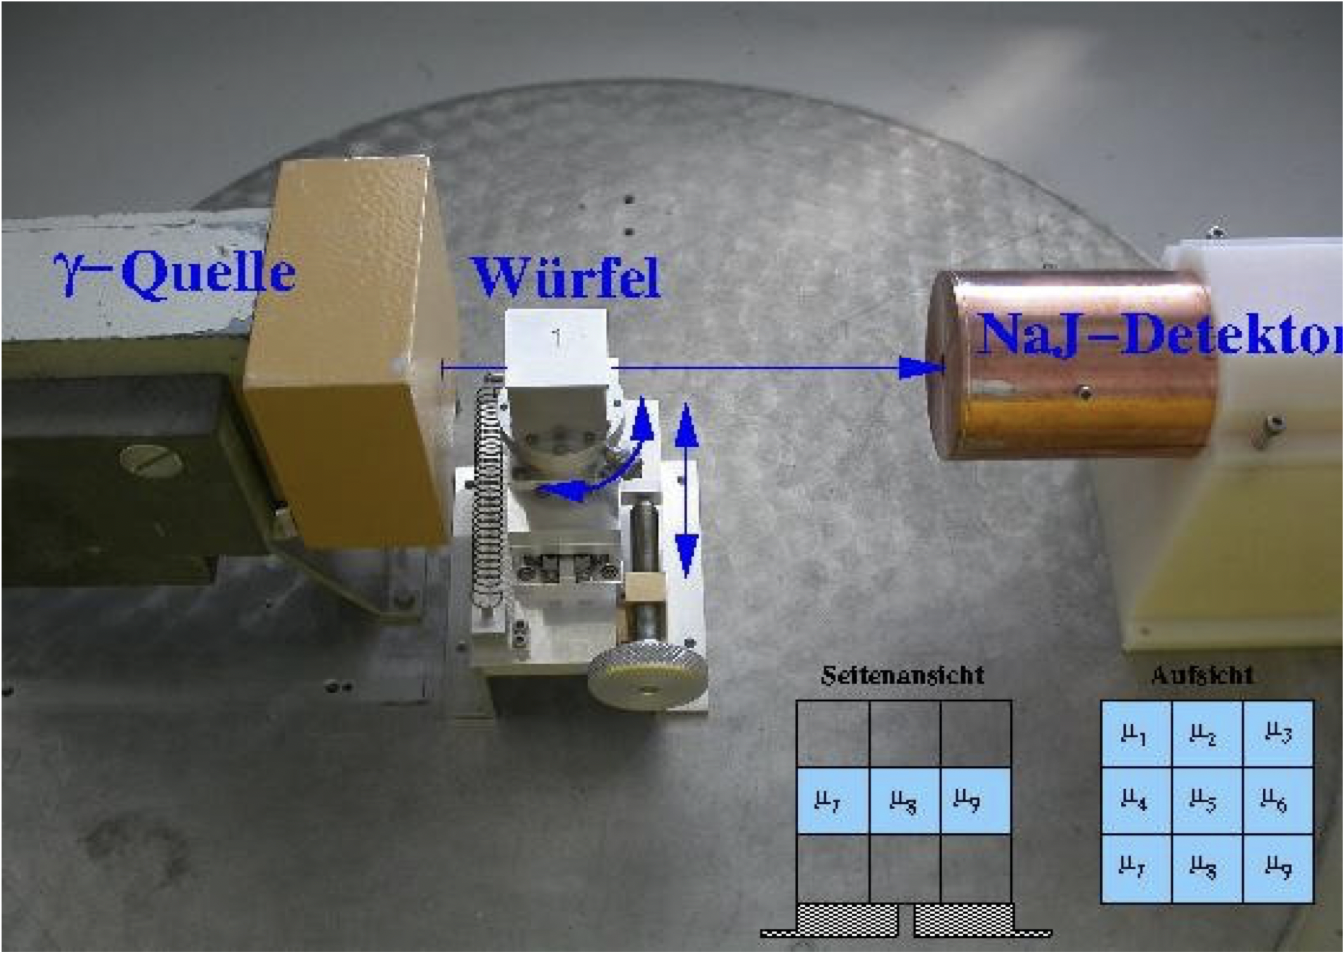
\includegraphics[width = 0.6\textwidth]{pictures/Aufbau.png}
          \caption{Der Aufbau zur Vermessung der Absorptionkoeffizienten unbekannter Materialien. Entnommen aus \cite{tu_dortmund_versuchsanleitung_2021-6}}
          \label{fig:Aufbau}
        \end{figure}
        Ein $^{137}\text{Cs}$-Strahler sendet aus einer kleinen Öffnung kollimierte $\gamma$-Strahlung aus.
        Diese passiert eine Halterung in der die zu untersuchenden Würfel eingebaut, bewegt und rotiert werden können.
        Diese Würfel bestehen aus $3\times3\times3$ Elementarwürfeln mit je $1\,\text{cm}$ Kantenlänge in einer dünnen Aluminiumhülle.
        Im Rahmen dieses Versuches wird nur die mittlere $3\times3$ Schicht der Würfel untersucht.
        Um die übriggebliebene Intensität, nach Durchqueren des Würfels, zu messen,
        trifft die Strahlung daraufhin auf einen anorganischen Szintillationsdetektor.
        Dabei werden die Atome des Szintillatormaterials angeregt, welche sich durch Emission eines Photons wieder abregen.
        Diese Photonen treffen auf einen Photomultiplier, welcher an einen Multichannelanalyzer angeschlossen ist,
        der die gemessenen Impulse der Größe nach in ein Histogramm einsortiert und dieses auf dem Computer ausgibt.
        Der gesamte Aufbau ist zusätzlich mit einer Wand aus Blei-Blöcken abgeschirmt.

        % Als Erstes wird eine Leermessung ohne eingespannten Würfel durchgeführt.
        Nun werden der Reihe nach vier verschiedene Würfel in der Halterung befestigt und nach der in Abbildung \ref{fig:Richtungen}
        gezeigten Projektion bestrahlt.
        Bei dem ersten Würfel handelt es sich lediglich um eine Hülle aus Aluminium.
        Die nächsten zwei Würfel sind zusätzlich homogen gefüllt.
        Diese werden jeweils aus sechs Richtungen ($I_1,...,I_6$) bestrahlt und
        die entsprechenden Absorptionsspektren aufgenommen.
        Als letztes wird ein Würfel unbekannter Zusammensetzung untersucht,
        indem dieser aus allen 12 Richtungen der Projektion aus Abbildung \ref{fig:Richtungen} bestrahlt wird.
        % \begin{figure}[h]
        %     \centering
        %     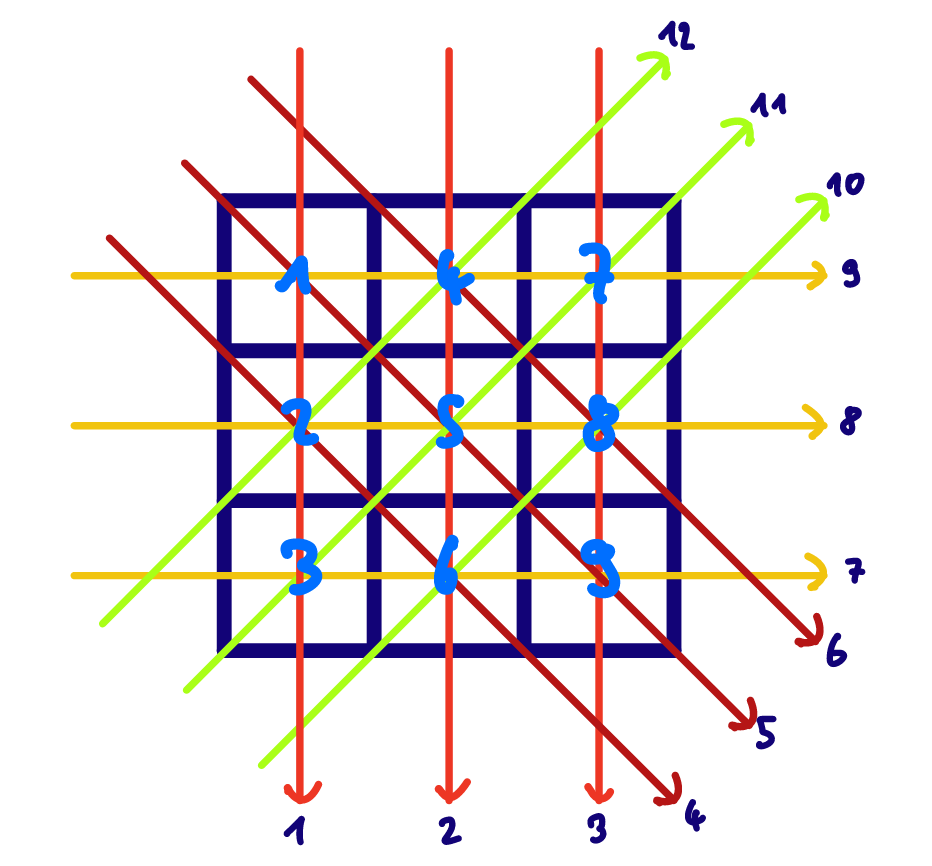
\includegraphics[width = 0.6\textwidth]{pictures/richtungen.png}
        %     \caption{Schematische Darstellung der Mittelschicht der Würfel. Die verschiedenen Bestrahlungsrichtungen sind ebenfalls eingetragen.}
        %     \label{fig:Projektion}
        %   \end{figure}
          

    %     Um die Spektrallinien und deren Aufspaltung zu vermessen, wird eine Cadmium-Spektrallampe innerhalb eines Elektromagnetens so platziert, dass das Licht der Lampe senkrecht zu den Magnetfeldlinien 
    %     beobachtet werden kann. Dieses ausgesendete Licht wird zunächst durch das Objetiv O kollimiert und anschließend durch die Kondensorlinse L$_1$ möglichst genau auf den Spalt S$_1$ abgebildet. Hinter 
    %     dem Spalt wird das Licht durch die Linse L$_2$ erneut kollimiert und durchläuft daraufhin ein Geradsichtprisma, in dem die Wellenlängenkomponenten aufgrund unterschiedlich starker Brechung räumlich 
    %     getrennt werden. Es ergeben sich eine grüne, blaue, dunkelblaue und rote Komponente. Die nun getrennten Komponenten durchlaufen einen Polarisationsfilter, der ermöglicht nur ausgewählte Übergänge zu 
    %     beobachten und werden durch die Linse L$_3$ auf einen weiteren Spalt S$_2$ fokussiert. Dieser ist verschiebbar, sodass eine ausgewählte Wellenlängenkomponenten den Spalt durchlaufen kann, während alle 
    %     anderen Komponenten blockiert werden. Zuletzt wird das Licht über die Linse L$_4$ auf die Lummer-Gehrcke-Platte fokussiert. Diese erzeugt ein Interferenzmuster, das über eine Digitalkamera aufgenommen 
    %     und aus dem die Wellenlänge des Lichts bestimmt werden kann.

    %     \FloatBarrier

    %     \begin{figure}[h]
    %       \centering
    %       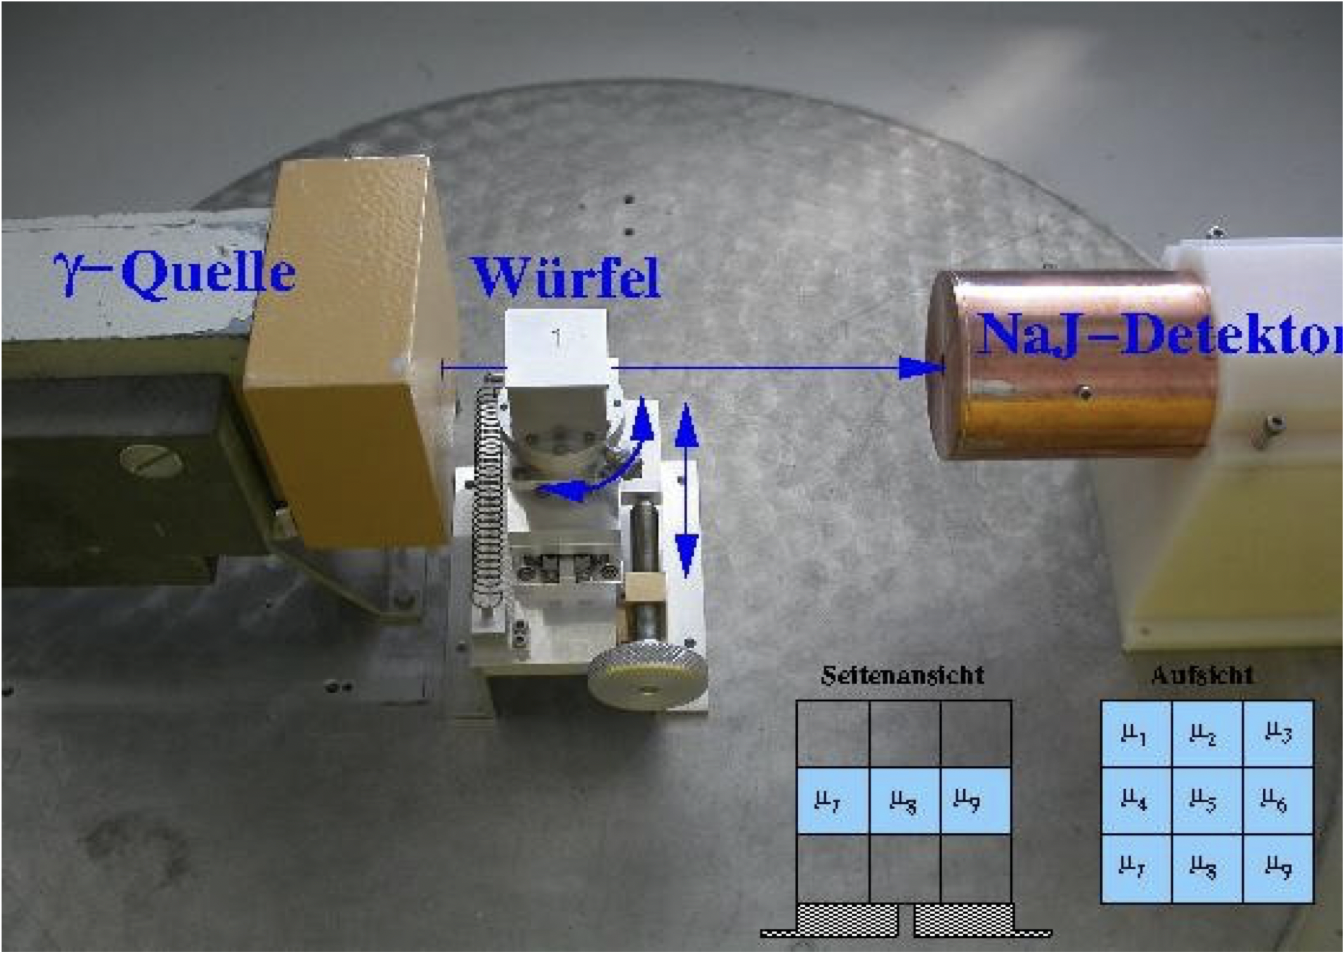
\includegraphics[width = 0.8\textwidth]{pictures/Aufbau.png}
    %       \caption{Der Aufbau zur Vermessung der Spektrallinien sowie deren Aufspaltung. Das Licht stammt aus einer Cadmium-Spektrallampe und die Spektrallinien werden durch einen Elektromagneten aufgespalten. Anschließend wird das Licht durch ein Geradsichtprisma räumlich in seine Wellenlängenkomponenten zerlegt. Die Komponenten können einzeln auf eine Lummer-Gehrcke-Platte abgebildet werden und erzeugen dort ein Interferenzbild.}
    %       \label{fig:Aufbau}
    %     \end{figure}
    
    %     \FloatBarrier

    

    % \subsection{Kalibrierung des Magnetfelds}
    %     Für die Auswertung der Aufspaltung ist die Kenntnis des angelegten Magnetfelds notwendigs. Da das Magnetfeld jedoch nicht gemessen werden kann, während die Spektrallampe in den Elektromagneten 
    %     eingesetzt ist, wird das Magnetfeld im Zentrum des Elektromagneten zunächst kalibriert. Dazu wird das Magnetfeld in Abhängigkeit vom angelegtem Spulenstrom mit einer Hall-Sonde im Bereich von 
    %     \SI{0.4}{\ampere} bis \SI{7.2}{\ampere} vermessen. So soll ein Zusammenhang zwischen Magnetfeldstärke und Stromstärke ermittelt werden, der es ermöglicht die angelegte Magnetfeldstärke über den 
    %     Spulenstrom zu berechnen.   

    % \subsection{Vermessung der Spektrallinienaufspaltung}
    %     \subsubsection*{Vermessung des normalen Zeeman-Effekts}
    %         Zur Vermessung des normalen Zeeman-Effekts wird die rote Spektrallinie untersucht. Dazu wird diese auf die Lummer-Gehrcke-Platte abgebildet und das Interferenzbild für vier Fälle aufgenommen.
            
    %         \begin{enumerate}
    %             \item I$_{\text{Spule}}$ = \SI{0}{\ampere}, $\qquad$    $\varphi_{\text{Pol}}$ = \SI{0}{\degree}
    %             \item I$_{\text{Spule}}$ = \SI{0}{\ampere}, $\qquad$    $\varphi_{\text{Pol}}$ = \SI{90}{\degree}
    %             \item I$_{\text{Spule}}$ = \SI{5}{\ampere}, $\qquad$    $\varphi_{\text{Pol}}$ = \SI{0}{\degree}
    %             \item I$_{\text{Spule}}$ = \SI{5}{\ampere}, $\qquad$    $\varphi_{\text{Pol}}$ = \SI{90}{\degree}
    %         \end{enumerate}

    %         In den ersten beiden Fällen liegt kein Magnetfeld an und die Spektrallinie sollte nicht aufgespalten sein. Im dritten und vierten Fall sind die Spektrallinien aufgespalten. Es sollte dennoch nur 
    %         im dritten Fall eine optische Aufspaltung erkennbar sein, da das Licht des normalen Übergangs hier nicht durch den Polarisationsfilter herausgefiltert wird.
            
            
    %     \subsubsection*{Vermessung des anormalen Zeeman-Effekts}
    %         Zur Vermessung des anormalen Zeeman-Effekts wird die blaue Spektrallinie untersucht. Diese wird wie die rote auf die Lummer-Gehrcke-Platte abgebildet und das Interferenzbild für folgende vier Fälle 
    %         aufgenommen. Hier ist der letzte Fall durch eine Magnetfeldstärke definiert, da die zugehörigen Daten aus einem externen Experiment übernommen werden mussten.
            
    %         \begin{enumerate}
    %             \item I$_{\text{Spule}}$ = \SI{0}{\ampere}, $\qquad$    $\varphi_{\text{Pol}}$ = \SI{0}{\degree}
    %             \item I$_{\text{Spule}}$ = \SI{0}{\ampere}, $\qquad$    $\varphi_{\text{Pol}}$ = \SI{90}{\degree}
    %             \item I$_{\text{Spule}}$ = \SI{2.6}{\ampere}, $\qquad$    $\varphi_{\text{Pol}}$ = \SI{0}{\degree}
    %             \item B$_{\text{Spule}}$ = \SI{1.009}{\tesla}, $\qquad$    $\varphi_{\text{Pol}}$ = \SI{90}{\degree}
    %         \end{enumerate}

    %         Erneut sollte für die ersten beiden Fällen keine Aufspaltung zu sehen sein. Im dritten und vierten Fall sind die Spektrallinien erneut aufgespalten. Bei dieser Beobachtung sollte die optische 
    %         Aufspaltung im Gegensatz zur Beobachtung des normalen Zeeman-Effekts im vierten Fall bei einem Polarisationswinkel von \SI{90}{\degree} zu sehen sein.
        
